\documentclass[tikz, border=3mm]{standalone}
\usetikzlibrary{chains,decorations.pathreplacing}

\begin{document}
    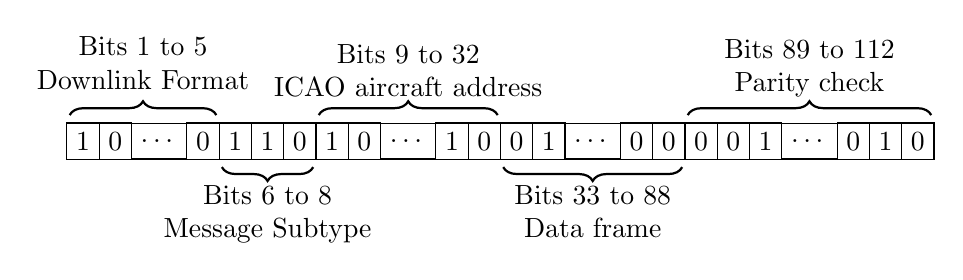
\begin{tikzpicture}[
node distance=0pt,
 start chain = A going right,
    X/.style = {rectangle, draw,% styles of nodes in string (chain)
                minimum width=2ex, minimum height=3ex,
                outer sep=0pt, on chain},
    B/.style = {decorate,
                decoration={brace, amplitude=5pt,
                pre=moveto,pre length=1pt,post=moveto,post length=1pt,
                raise=1mm,
                            #1}, % for mirroring of brace, if necessary
                thick},
    B/.default=mirror, % by default braces are mirrored
    C/.style = {decorate,
                decoration={brace, amplitude=5pt,
                pre=moveto,pre length=1pt,post=moveto,post length=1pt,
                raise=7mm,
                            #1}, % for mirroring of brace, if necessary
                thick},
    C/.default=mirror,
                        ]
%Sample Data
%10001101010010000100000011010110001000000010110011000011
%01110001110000110010110011100000010101110110000010011000

\foreach \i in {1,0,\ldots,0,1,1,0,1,0,\ldots,1,0,0,1,\ldots,0,0,0,0,1,\ldots,0,1,0}                        
    \node[X] {\i};

\draw[B=](A-1.north west) -- node[above=3mm,align=center] {Bits 1 to 5 \\ Downlink Format}(A-5.north west);
\draw[B] ( A-5.south west) -- node[below=2mm,align=center] {Bits 6 to 8\\ Message Subtype} ( A-7.south east);
\draw[B=](A-8.north west) -- node[above=2mm,align=center] {Bits 9 to 32\\ ICAO aircraft address}(A-13.north west);
\draw[B](A-13.south west) -- node[below=2mm,align=center] {Bits 33 to 88 \\ Data frame}(A-17.south east);
\draw[B=](A-18.north west) -- node[above=2mm,align=center] {Bits 89 to 112\\ Parity check}(A-24.north east);

\end{tikzpicture}
\end{document}
